%!TEX program = xelatex

\documentclass{ctexart}
	\usepackage{amsmath}
	\usepackage{amssymb}
	\usepackage{changepage}
    \usepackage{pgf}
    \usepackage{tikz}
    \usetikzlibrary{arrows,automata}
    % \usepackage[latin1]{inputenc}
    \usepackage{verbatim}
    \title{Solution for Homework1}
    \author{徐翔哲(161250170)} 
    
\begin{document}
\maketitle
\newpage
\section{PROBLEM 1}
\subsection{a}

Firstly, we can get the automata as follows.\\

% 1-1-1
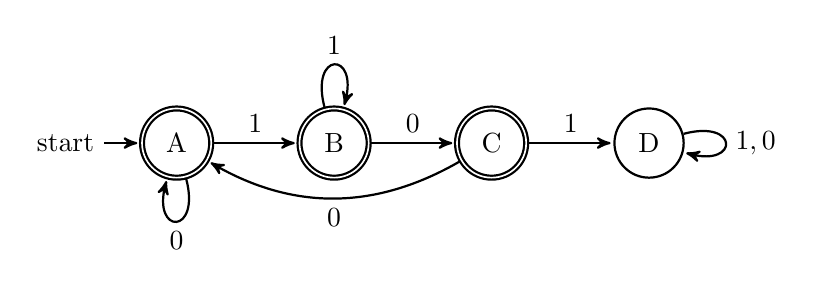
\begin{tikzpicture}
	[->,>=stealth',shorten >=1pt,auto,node distance=2cm,
		thick,base node/.style={circle,draw,minimum size=16pt}, real node/.style={double,circle,draw,minimum size=35pt}]

	\node[initial, initial text={start},accepting, state] (A) {A};
	\node[accepting, state] (B)[right of = A] {B};
	\node[accepting, state] (C)[right of = B] {C};
	\node[state] (D)[right of = C] {D};

	% \node[initial,initial text={}, accepting, state] (1) {$\epsilon$};
	% \node[state](2)[right of=1 ]{$51$}[above];

	\path[]
	(A) edge [loop below]   node {$0$}  (A)
	edge                node {$1$}     (B)
	(B) edge [loop above]   node {$1$}  (B)
	edge                node {$0$}  (C)
	(C) edge [bend left]   node {$0$}  (A)
	edge                node {$1$}  (D)
	(D) edge [loop right]   node {$1,0$} (D)
	;


\end{tikzpicture}

Then we just delete state D since it contributes nothing to the accepted strings.\\

% 1-1-2
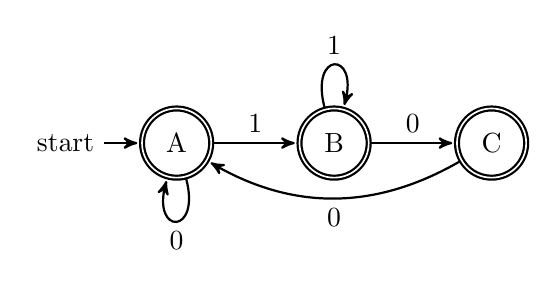
\begin{tikzpicture}
	[->,>=stealth',shorten >=1pt,auto,node distance=2cm,
		thick,base node/.style={circle,draw,minimum size=16pt}, real node/.style={double,circle,draw,minimum size=35pt}]


	\node[initial, initial text={start},accepting, state] (A) {A};
	\node[accepting, state] (B)[right of = A] {B};
	\node[accepting, state] (C)[right of = B] {C};

	\path[]
	(A) edge [loop below]   node {$0$}  (A)
	edge                node {$1$}     (B)
	(B) edge [loop above]   node {$1$}  (B)
	edge                node {$0$}  (C)
	(C) edge [bend left]   node {$0$}  (A)
	;
\end{tikzpicture}

First, we pick A as the accepting state. Then we get $(0^*+11^*00)^*$\\

% branch1-1
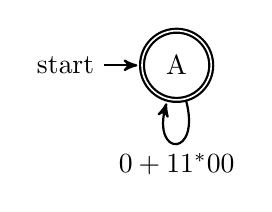
\begin{tikzpicture}
	[->,>=stealth',shorten >=1pt,auto,node distance=2cm,
		thick,base node/.style={circle,draw,minimum size=16pt}, real node/.style={double,circle,draw,minimum size=35pt}]


	\node[initial, initial text={start},accepting, state] (A) {A};

	\path[]
	(A) edge [loop below]   node {$0+11^*00$}  (A)
	% edge                node {$1$}     (B)
	% (B) edge [loop above]   node {$1$}  (B)
	%     edge                node {$0$}  (C)
	% (C) edge [bend left]   node {$0$}  (A)
	;
\end{tikzpicture}

Then we choose state C as the accepting state. Then we get $(0+11^*00)^*11^*0$\\

% branch 1-2
\begin{tikzpicture}
	[->,>=stealth',shorten >=1pt,auto,node distance=2cm,
		thick,base node/.style={circle,draw,minimum size=16pt}, real node/.style={double,circle,draw,minimum size=35pt}]


	\node[initial, initial text={start},accepting, state] (A) {A};
	\node[accepting, state] (C)[right of = B] {C};

	\path[]
	(A) edge [loop below]   node {$0$}  (A)
	edge                node {$11^*0$}     (C)
	(C) edge [bend left]   node {$0$}  (A)
	;
\end{tikzpicture}

Finally, we choose B as the accepting state. Then we get $(0+11^*00)^*11^* $\\
% branch 2
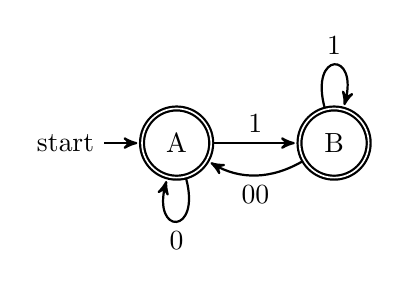
\begin{tikzpicture}
	[->,>=stealth',shorten >=1pt,auto,node distance=2cm,
		thick,base node/.style={circle,draw,minimum size=16pt}, real node/.style={double,circle,draw,minimum size=35pt}]


	\node[initial, initial text={start},accepting, state] (A) {A};
	\node[accepting, state] (B)[right of = A] {B};

	\path[]
	(A) edge [loop below]   node {$0$}  (A)
	edge                node {$1$}     (B)
	(B) edge [loop above]   node {$1$}  (B)
	edge [bend left]    node {$00$}  (A)
	;
\end{tikzpicture}

In all, we have $(0^*+11^*00)^* + (0+11^*00)^*11^*0 + (0+11^*00)^*11^* $

\subsection{b}

First, we get the DFA as follows:\\

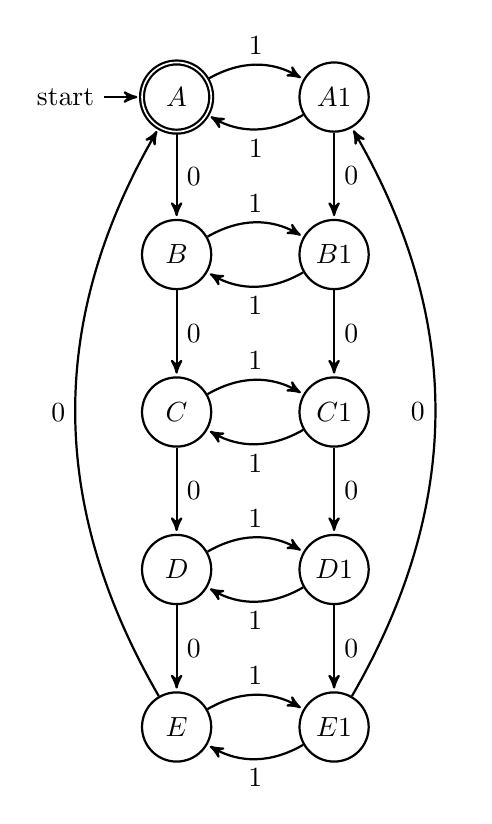
\begin{tikzpicture}
	[->,>=stealth',shorten >=1pt,auto,node distance=2cm,
		thick,base node/.style={circle,draw,minimum size=16pt}, real node/.style={double,circle,draw,minimum size=35pt}]

	\node[initial, initial text={start}, accepting, state] (A) {$A$};
	\node[state]    (A1)    [right of = A]  {$A1$};
	\node[state]    (B)     [below of = A]  {$B$};
	\node[state]    (B1)     [below of = A1]  {$B1$};
	\node[state]    (C)     [below of = B]  {$C$};
	\node[state]    (C1)     [below of = B1]  {$C1$};
	\node[state]    (D)     [below of = C]  {$D$};
	\node[state]    (D1)     [below of = C1]  {$D1$};
	\node[state]    (E)     [below of = D]  {$E$};
	\node[state]    (E1)     [below of = D1]  {$E1$};

	\path[]
	(A) edge [bend left]   node {$1$}  (A1)
	edge    node {$0$}  (B)
	(A1) edge [bend left]  node {$1$}  (A)
	edge    node {$0$}  (B1)
	(B) edge [bend left]   node {$1$}  (B1)
	edge    node {$0$}  (C)

	(B1) edge [bend left]  node {$1$}  (B)
	edge    node {$0$}  (C1)
	(C) edge [bend left]   node {$1$}  (C1)
	edge    node {$0$}  (D)
	(C1) edge [bend left]  node {$1$}  (C)
	edge    node {$0$}  (D1)
	(D) edge [bend left]   node {$1$}  (D1)
	edge    node {$0$}  (E)
	(D1) edge [bend left]  node {$1$}  (D)
	edge    node {$0$}  (E1)
	(E) edge [bend left]   node {$1$}  (E1)
	edge [bend left]   node {$0$}  (A)
	(E1) edge [bend left]  node {$1$}  (E)
	edge [bend right]   node {$0$}  (A1)

	;

\end{tikzpicture}\\

Then we delete state B1.\\


\begin{tikzpicture}
	[->,>=stealth',shorten >=1pt,auto,node distance=2cm,
		thick,base node/.style={circle,draw,minimum size=16pt}, real node/.style={double,circle,draw,minimum size=35pt}]

	\node[initial, initial text={start}, accepting, state] (A) {$A$};
	\node[state]    (A1)    [right of = A]  {$A1$};
	\node[state]    (B)     [below of = A]  {$B$};
	% \node[state]    (B1)     [below of = A1]  {$B1$};
	\node[state]    (C)     [below of = B]  {$C$};
	\node[state]    (C1)     [below of = B1]  {$C1$};
	\node[state]    (D)     [below of = C]  {$D$};
	\node[state]    (D1)     [below of = C1]  {$D1$};
	\node[state]    (E)     [below of = D]  {$E$};
	\node[state]    (E1)     [below of = D1]  {$E1$};

	\path[]
	(A) edge [bend left]   node {$1$}  (A1)
	edge    node {$0$}  (B)
	(A1) edge [bend left]  node {$1$}  (A)
	edge    node {$01$}  (B)
	edge    node {$00$}  (C1)
	(B) edge [loop right]   node {$11$}  (B)
	edge    node {$0$}  (C)
	edge    node {$10$}  (C1)

	% (B1) edge [bend left]  node {$1$}  (B)
	(C) edge [bend left]   node {$1$}  (C1)
	edge    node {$0$}  (D)
	(C1) edge [bend left]  node {$1$}  (C)
	edge    node {$0$}  (D1)
	(D) edge [bend left]   node {$1$}  (D1)
	edge    node {$0$}  (E)
	(D1) edge [bend left]  node {$1$}  (D)
	edge    node {$0$}  (E1)
	(E) edge [bend left]   node {$1$}  (E1)
	edge [bend left]   node {$0$}  (A)
	(E1) edge [bend left]  node {$1$}  (E)
	edge [bend right]   node {$0$}  (A1)

	;

\end{tikzpicture}\\

Then we delete state C.\\

\begin{tikzpicture}
	[->,>=stealth',shorten >=1pt,auto,node distance=2cm,
		thick,base node/.style={circle,draw,minimum size=16pt}, real node/.style={double,circle,draw,minimum size=35pt}]

	\node[initial, initial text={start}, accepting, state] (A) {$A$};
	\node[state]    (A1)    [right of = A]  {$A1$};
	\node[state]    (B)     [below of = A]  {$B$};
	% \node[state]    (B1)     [below of = A1]  {$B1$};
	% \node[state]    (C)     [below of = B]  {$C$};
	\node[state]    (C1)     [below of = B1]  {$C1$};
	\node[state]    (D)     [below of = C]  {$D$};
	\node[state]    (D1)     [below of = C1]  {$D1$};
	\node[state]    (E)     [below of = D]  {$E$};
	\node[state]    (E1)     [below of = D1]  {$E1$};

	\path[]
	(A) edge [bend left]   node {$1$}  (A1)
	edge    node {$0$}  (B)
	(A1) edge [bend left]  node {$1$}  (A)
	edge    node {$01$}  (B)
	edge    node {$00$}  (C1)
	(B) edge [loop right]   node {$11$}  (B)
	% edge    node {$0$}  (C)
	edge [bend right]   node {$10+01$}  (C1)
	edge  [bend right]  node {$00$}  (D)

	% (B1) edge [bend left]  node {$1$}  (B)
	(C1) edge [loop left]   node {$11$}  (C1)
	edge    node {$10$}  (D)
	(C1) edge    node {$0$}  (D1)
	(D) edge [bend left]   node {$1$}  (D1)
	edge    node {$0$}  (E)
	(D1) edge [bend left]  node {$1$}  (D)
	edge    node {$0$}  (E1)
	(E) edge [bend left]   node {$1$}  (E1)
	edge [bend left]   node {$0$}  (A)
	(E1) edge [bend left]  node {$1$}  (E)
	edge [bend right]   node {$0$}  (A1)

	;

\end{tikzpicture}\\

Then we delete state D1.\\

\begin{tikzpicture}
	[->,>=stealth',shorten >=1pt,auto,node distance=2cm,
		thick,base node/.style={circle,draw,minimum size=16pt}, real node/.style={double,circle,draw,minimum size=35pt}]

	\node[initial, initial text={start}, accepting, state] (A) {$A$};
	\node[state]    (A1)    [right of = A]  {$A1$};
	\node[state]    (B)     [below of = A]  {$B$};
	% \node[state]    (B1)     [below of = A1]  {$B1$};
	% \node[state]    (C)     [below of = B]  {$C$};
	\node[state]    (C1)     [below of = B1]  {$C1$};
	\node[state]    (D)     [below of = C]  {$D$};
	% \node[state]    (D1)     [below of = C1]  {$D1$};
	\node[state]    (E)     [below of = D]  {$E$};
	\node[state]    (E1)     [below of = D1]  {$E1$};

	\path[]
	(A) edge [bend left]   node {$1$}  (A1)
	edge    node {$0$}  (B)
	(A1) edge [bend left]  node {$1$}  (A)
	edge    node {$01$}  (B)
	edge    node {$00$}  (C1)
	(B) edge [loop right]   node {$11$}  (B)
	% edge    node {$0$}  (C)
	edge [bend right]   node {$10+01$}  (C1)
	edge  [bend right]  node {$00$}  (D)

	% (B1) edge [bend left]  node {$1$}  (B)
	(C1) edge [loop left]   node {$11$}  (C1)
	edge    node {$10+01$}  (D)
	edge    node {$00$}  (E1)
	% (C1) edge    node {$0$}  (D1)
	(D) edge [loop right]   node {$11$}  (D)
	edge    node {$10$}  (E1)
	edge    node {$0$}  (E)
	% (D1) edge [bend left]  node {$1$}  (D)
	% edge    node {$0$}  (E1)
	(E) edge [bend left]   node {$1$}  (E1)
	edge [bend left]   node {$0$}  (A)
	(E1) edge [bend left]  node {$1$}  (E)
	edge [bend right]   node {$0$}  (A1)

	;

\end{tikzpicture}\\

Then we delete state E.\\


\begin{tikzpicture}
	[->,>=stealth',shorten >=1pt,auto,node distance=2cm,
		thick,base node/.style={circle,draw,minimum size=16pt}, real node/.style={double,circle,draw,minimum size=35pt}]

	\node[initial, initial text={start}, accepting, state] (A) {$A$};
	\node[state]    (A1)    [right of = A]  {$A1$};
	\node[state]    (B)     [below of = A]  {$B$};
	% \node[state]    (B1)     [below of = A1]  {$B1$};
	% \node[state]    (C)     [below of = B]  {$C$};
	\node[state]    (C1)     [below of = B1]  {$C1$};
	\node[state]    (D)     [below of = C]  {$D$};
	% \node[state]    (D1)     [below of = C1]  {$D1$};
	% \node[state]    (E)     [below of = D]  {$E$};
	\node[state]    (E1)     [below of = D1]  {$E1$};

	\path[]
	(A) edge [bend left]   node {$1$}  (A1)
	edge    node {$0$}  (B)
	(A1) edge [bend left]  node {$1$}  (A)
	edge    node {$01$}  (B)
	edge    node {$00$}  (C1)
	(B) edge [loop right]   node {$11$}  (B)
	% edge    node {$0$}  (C)
	edge [bend right]   node {$10+01$}  (C1)
	edge  [bend right]  node {$00$}  (D)

	% (B1) edge [bend left]  node {$1$}  (B)
	(C1) edge [loop left]   node {$11$}  (C1)
	edge    node {$10+01$}  (D)
	edge    node {$00$}  (E1)
	% (C1) edge    node {$0$}  (D1)
	(D) edge [loop right]   node {$11$}  (D)
	edge    node {$10+01$}  (E1)
	edge [bend left]   node {$00$}  (A)

	% edge    node {$0$}  (E)
	% (D1) edge [bend left]  node {$1$}  (D)
	% edge    node {$0$}  (E1)
	% (E) edge [bend left]   node {$1$}  (E1)
	% edge [bend left]   node {$0$}  (A)
	(E1) edge [loop left]  node {$11$}  (E1)
	edge [bend left]   node {$10$}  (A)

	edge [bend right]   node {$0$}  (A1)

	;

\end{tikzpicture}\\

Then we delete state B where $L_1=10+01$.\\

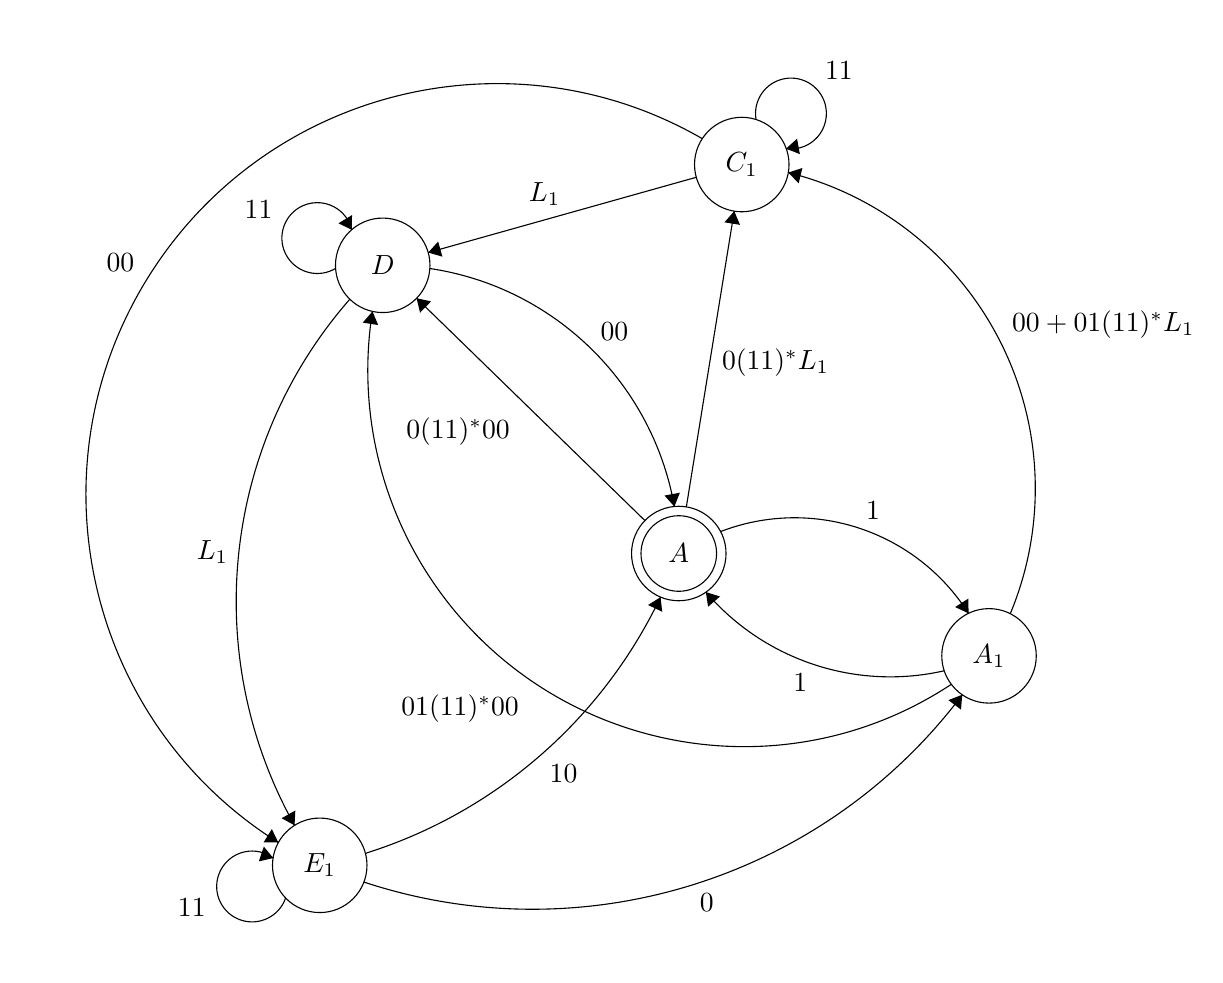
\begin{tikzpicture}[scale=0.2]
	\tikzstyle{every node}+=[inner sep=0pt]
	\draw [black] (41,-32.8) circle (3);
	\draw (41,-32.8) node {$A$};
	\draw [black] (41,-32.8) circle (2.4);
	\draw [black] (60.7,-39.3) circle (3);
	\draw (60.7,-39.3) node {$A_1$};
	\draw [black] (18.2,-52.6) circle (3);
	\draw (18.2,-52.6) node {$E_1$};
	\draw [black] (45,-8.1) circle (3);
	\draw (45,-8.1) node {$C_1$};
	\draw [black] (22.2,-14.5) circle (3);
	\draw (22.2,-14.5) node {$D$};
	\draw [black] (43.65,-31.409) arc (111.12351:32.35595:13.067);
	\fill [black] (59.4,-36.6) -- (59.39,-35.66) -- (58.55,-36.2);
	\draw (53.34,-30.65) node [above] {$1$};
	\draw [black] (45.908,-5.253) arc (190.05134:-97.94866:2.25);
	\draw (51.17,-2.76) node [above] {$11$};
	\fill [black] (47.81,-7.09) -- (48.69,-7.44) -- (48.51,-6.46);
	\draw [black] (19.218,-14.69) arc (301.38014:13.38014:2.25);
	\draw (15.23,-10.98) node [left] {$11$};
	\fill [black] (20.24,-12.25) -- (20.25,-11.31) -- (19.39,-11.83);
	\draw [black] (16.037,-54.662) arc (-18.64598:-306.64598:2.25);
	\draw (10.99,-55.26) node [left] {$11$};
	\fill [black] (15.25,-52.14) -- (14.65,-51.41) -- (14.33,-52.35);
	\draw [black] (47.954,-8.611) arc (76.02951:-22.60596:20.677);
	\fill [black] (47.95,-8.61) -- (48.61,-9.29) -- (48.85,-8.32);
	\draw (62.13,-18.27) node [right] {$00+01(11)^*L_1$};
	\draw [black] (41.48,-29.84) -- (44.52,-11.06);
	\fill [black] (44.52,-11.06) -- (43.9,-11.77) -- (44.89,-11.93);
	\draw (43.71,-20.67) node [right] {$0(11)^*L_1$};
	\draw [black] (58.307,-41.106) arc (-56.55381:-189.02189:23.89);
	\fill [black] (21.55,-17.43) -- (20.93,-18.14) -- (21.91,-18.29);
	\draw (27.11,-41.76) node [below] {$01(11)^*00$};
	\draw [black] (57.858,-40.246) arc (-77.1518:-139.36873:15.426);
	\fill [black] (42.72,-35.25) -- (42.86,-36.18) -- (43.62,-35.53);
	\draw (48.71,-40.39) node [below] {$1$};
	\draw [black] (25.19,-14.701) arc (81.51747:10.0268:18.548);
	\fill [black] (40.72,-29.82) -- (41.07,-28.94) -- (40.09,-29.12);
	\draw (36.91,-19.28) node [above] {$00$};
	\draw [black] (38.85,-30.71) -- (24.35,-16.59);
	\fill [black] (24.35,-16.59) -- (24.57,-17.51) -- (25.27,-16.79);
	\draw (26.98,-24.13) node [below] {$0(11)^*00$};
	\draw [black] (59.004,-41.773) arc (-36.96172:-108.28418:34.149);
	\fill [black] (59,-41.77) -- (58.12,-42.11) -- (58.92,-42.71);
	\draw (42.78,-54.37) node [below] {$0$};
	\draw [black] (42.11,-8.91) -- (25.09,-13.69);
	\fill [black] (25.09,-13.69) -- (25.99,-13.95) -- (25.72,-12.99);
	\draw (32.48,-10.72) node [above] {$L_1$};
	\draw [black] (15.573,-51.154) arc (-122.12951:-299.98716:26.094);
	\fill [black] (15.57,-51.15) -- (15.16,-50.3) -- (14.63,-51.15);
	\draw (6.46,-14.33) node [left] {$00$};
	\draw [black] (39.842,-35.566) arc (-25.49039:-72.56614:31.076);
	\fill [black] (39.84,-35.57) -- (39.05,-36.07) -- (39.95,-36.5);
	\draw (33.68,-46.15) node [below] {$10$};
	\draw [black] (16.603,-50.062) arc (-150.77208:-221.21462:29.125);
	\fill [black] (16.6,-50.06) -- (16.65,-49.12) -- (15.78,-49.61);
	\draw (12.41,-32.7) node [left] {$L_1$};
\end{tikzpicture}\\


Then we delete E1.\\

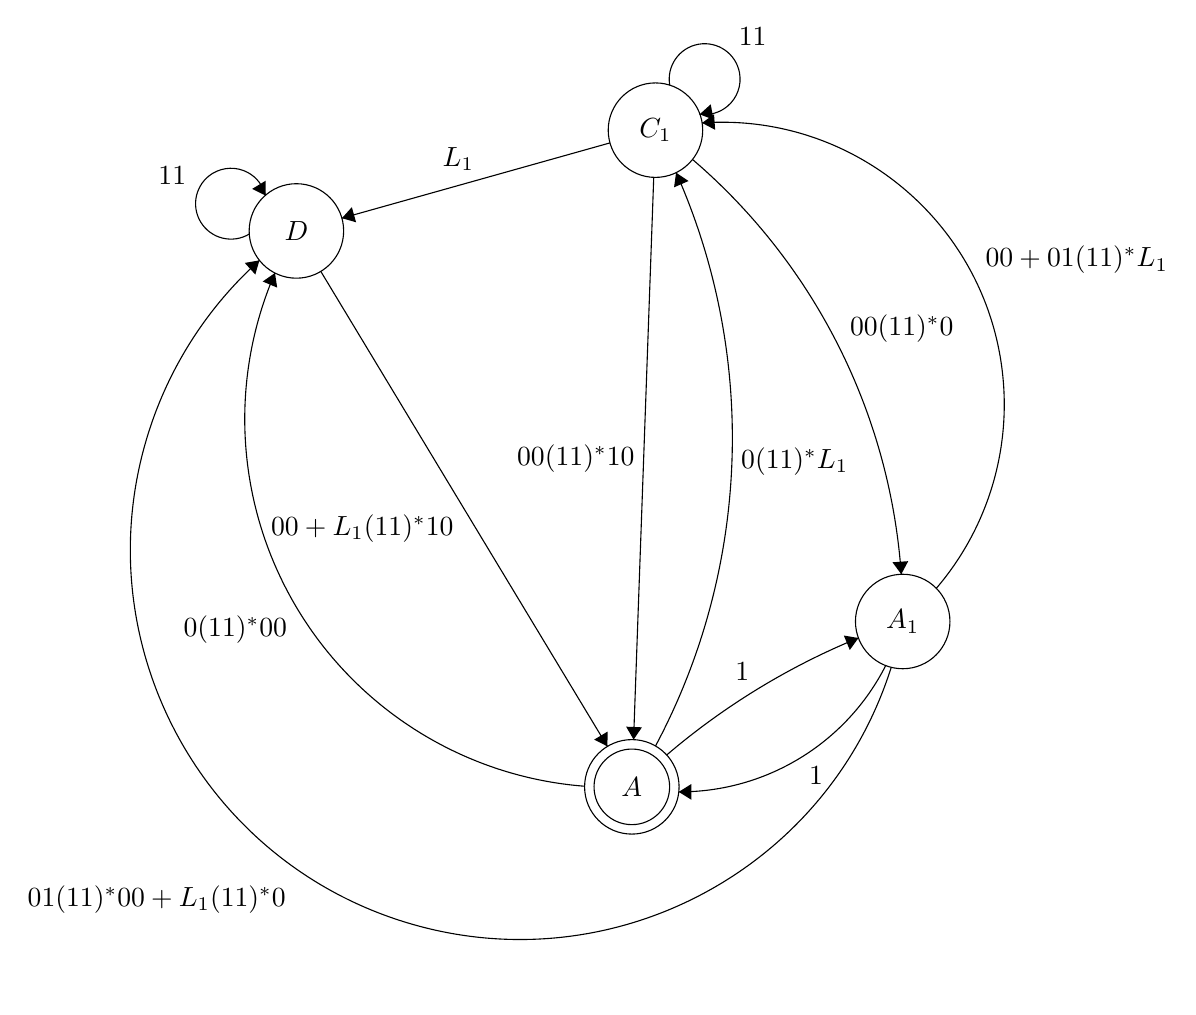
\begin{tikzpicture}[scale=0.2]
	\tikzstyle{every node}+=[inner sep=0pt]
	\draw [black] (43.5,-49.8) circle (3);
	\draw (43.5,-49.8) node {$A$};
	\draw [black] (43.5,-49.8) circle (2.4);
	\draw [black] (60.7,-39.3) circle (3);
	\draw (60.7,-39.3) node {$A_1$};
	\draw [black] (45,-8.1) circle (3);
	\draw (45,-8.1) node {$C_1$};
	\draw [black] (22.2,-14.5) circle (3);
	\draw (22.2,-14.5) node {$D$};
	\draw [black] (45.714,-47.777) arc (130.50667:112.29855:45.072);
	\fill [black] (57.89,-40.35) -- (56.96,-40.19) -- (57.34,-41.11);
	\draw (50.51,-43.08) node [above] {$1$};
	\draw [black] (45.908,-5.253) arc (190.05134:-97.94866:2.25);
	\draw (51.17,-2.76) node [above] {$11$};
	\fill [black] (47.81,-7.09) -- (48.69,-7.44) -- (48.51,-6.46);
	\draw [black] (19.218,-14.69) arc (301.38014:13.38014:2.25);
	\draw (15.23,-10.98) node [left] {$11$};
	\fill [black] (20.24,-12.25) -- (20.25,-11.31) -- (19.39,-11.83);
	\draw [black] (47.961,-7.641) arc (94.0212:-40.59765:17.931);
	\fill [black] (47.96,-7.64) -- (48.79,-8.08) -- (48.72,-7.09);
	\draw (65.93,-16.35) node [right] {$00+01(11)^*L_1$};
	\draw [black] (46.314,-10.796) arc (23.91032:-28.03054:41.598);
	\fill [black] (46.31,-10.8) -- (46.18,-11.73) -- (47.1,-11.33);
	\draw (50.41,-29.16) node [right] {$0(11)^*L_1$};
	\draw [black] (59.972,-42.208) arc (-17.53501:-228.04068:24.732);
	\fill [black] (19.85,-16.37) -- (18.92,-16.53) -- (19.59,-17.27);
	\draw (13.33,-56.05) node [below] {$01(11)^*00+L_1(11)^*0$};
	\draw [black] (59.623,-42.094) arc (-26.93721:-90.25757:14.671);
	\fill [black] (46.48,-50.12) -- (47.28,-50.62) -- (47.28,-49.62);
	\draw (55.19,-48.47) node [below] {$1$};
	\draw [black] (23.75,-17.07) -- (41.95,-47.23);
	\fill [black] (41.95,-47.23) -- (41.96,-46.29) -- (41.11,-46.8);
	\draw (32.21,-33.42) node [left] {$00+L_1(11)^*10$};
	\draw [black] (40.502,-49.761) arc (-94.41412:-203.37236:23.384);
	\fill [black] (20.84,-17.17) -- (20.06,-17.71) -- (20.98,-18.1);
	\draw (21.64,-39.79) node [left] {$0(11)^*00$};
	\draw [black] (42.11,-8.91) -- (25.09,-13.69);
	\fill [black] (25.09,-13.69) -- (25.99,-13.95) -- (25.72,-12.99);
	\draw (32.48,-10.72) node [above] {$L_1$};
	\draw [black] (44.89,-11.1) -- (43.61,-46.8);
	\fill [black] (43.61,-46.8) -- (44.14,-46.02) -- (43.14,-45.98);
	\draw (43.7,-28.94) node [left] {$00(11)^*10$};
	\draw [black] (47.353,-9.96) arc (49.41298:4.01057:38.205);
	\fill [black] (60.61,-36.3) -- (61.05,-35.47) -- (60.05,-35.54);
	\draw (57.32,-20.69) node [right] {$00(11)^*0$};
\end{tikzpicture}\\

Then we can delete state C1. And
$$
	L_1=10+01
$$
$$
	L_2=00+01(11)^*L_1\\
$$
$$
	L_3=00(11)^*10\\
$$\\


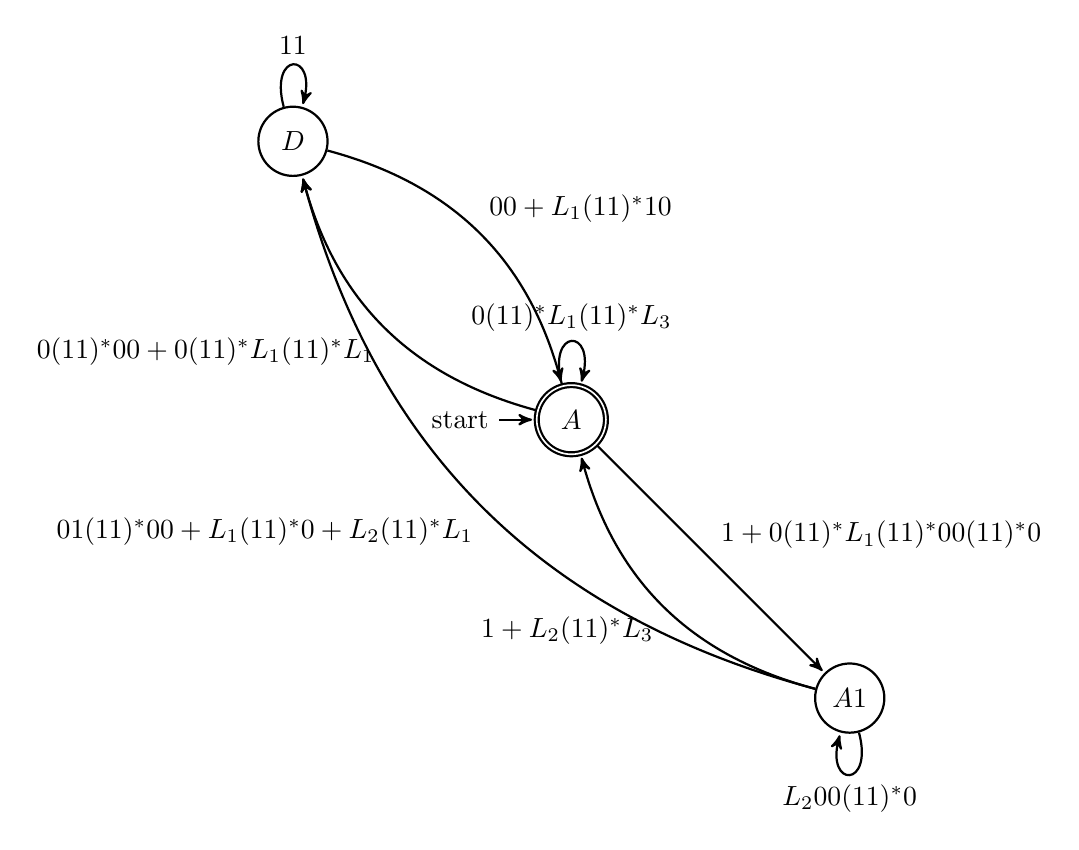
\begin{tikzpicture}
	[->,>=stealth',shorten >=1pt,auto,node distance=5cm,
		thick,base node/.style={circle,draw,minimum size=16pt}, real node/.style={double,circle,draw,minimum size=35pt}]

	\node[initial, initial text={start}, accepting, state] (A) {$A$};
	\node[state]    (A1)    [below right of = A]  {$A1$};
	% \node[state]    (B)     [below of = A]  {$B$};
	% \node[state]    (B1)     [below of = A1]  {$B1$};
	% \node[state]    (C)     [below of = B]  {$C$};
	% \node[state]    (C1)     [below of = B1]  {$C1$};
	\node[state]    (D)     [above left of = A]  {$D$};
	% \node[state]    (D1)     [below of = C1]  {$D1$};
	% \node[state]    (E)     [below of = D]  {$E$};
	% \node[state]    (E1)     [below of = D1]  {$E1$};

	\path[]
	(A) edge    node {$1+0(11)^*L_1(11)^*00(11)^*0$}  (A1)
	(A) edge [loop above]   node {$0(11)^*L_1(11)^*L_3$}  (A)
	(A1) edge [bend left]   node {$1+L_2(11)^*L_3$}  (A)
	(A1) edge [loop below]   node {$L_200(11)^*0 $}  (A1)
	(A1) edge [bend left]   node {$01(11)^*00+L_1(11)^*0+L_2(11)^*L_1 $}  (D)
	(D) edge [loop above]   node {$11$}  (D)
	(D) edge [bend left]   node {$00+L_1(11)^*10$}  (A)
	(A) edge [bend left]   node {$0(11)^*00+0(11)^*L_1(11)^*L_1 $}  (D)


	;

\end{tikzpicture}\\

Finally,
\[R=0(11)^*L_1(11)^*L_3+L_5(11)^*(00+L_1(11)^*10) \]
\[S=1+L_2(11)^*L_3+L_4(11)^*(00+L_1(11)^*10) \]
\[T=L_200(11)^*0 \]
\[L_1=10+01 \]
\[L_2=00+01(11)^*L_1 \]
\[L_3=00(11)^*10 \]
\[L_4=01(11)^*00+L_1(11)^*0+L_2(11)^*L_1 \]
\[L_5=0(11)^*00+0(11)^*L_1(11)^*L_1 \]
\[L_6=1+0(11)^*L_1(11)^*00(11)^*0 \]

And the answer should be $(R+L_6T^*S)^*$.\\

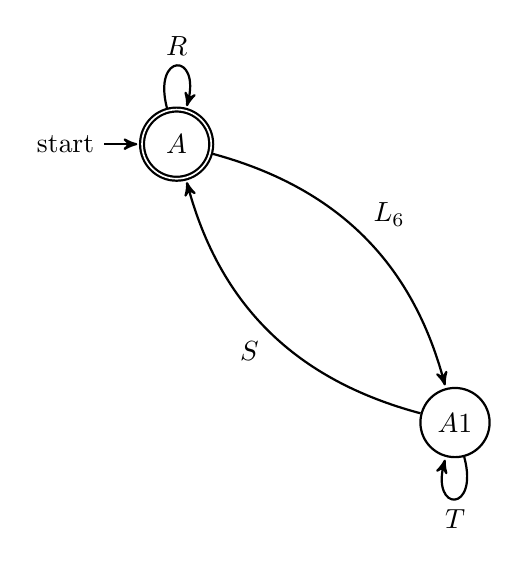
\begin{tikzpicture}
	[->,>=stealth',shorten >=1pt,auto,node distance=5cm,
		thick,base node/.style={circle,draw,minimum size=16pt}, real node/.style={double,circle,draw,minimum size=35pt}]

	\node[initial, initial text={start}, accepting, state] (A) {$A$};
	\node[state]    (A1)    [below right of = A]  {$A1$};
	% \node[state]    (B)     [below of = A]  {$B$};
	% \node[state]    (B1)     [below of = A1]  {$B1$};
	% \node[state]    (C)     [below of = B]  {$C$};
	% \node[state]    (C1)     [below of = B1]  {$C1$};
	% \node[state]    (D)     [above left of = A]  {$D$};
	% \node[state]    (D1)     [below of = C1]  {$D1$};
	% \node[state]    (E)     [below of = D]  {$E$};
	% \node[state]    (E1)     [below of = D1]  {$E1$};

	\path[]
	(A) edge [loop above]   node {$R$}  (A)
	(A) edge [bend left]   node {$L_6$}  (A1)
	(A1) edge [bend left]   node {$S$}  (A)
	(A1) edge [loop below]   node {$T $}  (A1)
	;

\end{tikzpicture}\\

\subsection{c}

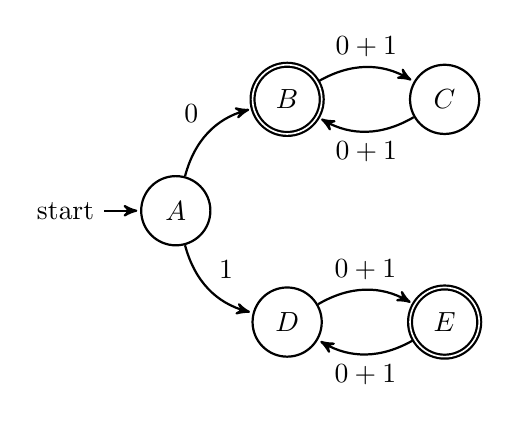
\begin{tikzpicture}
	[->,>=stealth',shorten >=1pt,auto,node distance=2cm,
		thick,base node/.style={circle,draw,minimum size=16pt}, real node/.style={double,circle,draw,minimum size=35pt}]

	\node[initial, initial text={start}, state] (A) {$A$};
	\node[accepting, state]    (B)     [above right of = A]  {$B$};
	\node[state]    (C)     [right of = B]  {$C$};
	\node[ state]    (D)     [below right of = A]  {$D$};
	\node[accepting, state]    (E)     [right of = D]  {$E$};

	\path[]
	(A) edge [bend left]   node {$0$}  (B)
	(A) edge [bend right]   node {$1$}  (D)
	(B) edge [bend left]   node {$0+1$}  (C)
	(C) edge [bend left]   node {$0+1$}  (B)
	(D) edge [bend left]   node {$0+1$}  (E)
	(E) edge [bend left]   node {$0+1$}  (D)

	;

\end{tikzpicture}\\

It can be simplified to the following DFA.\\

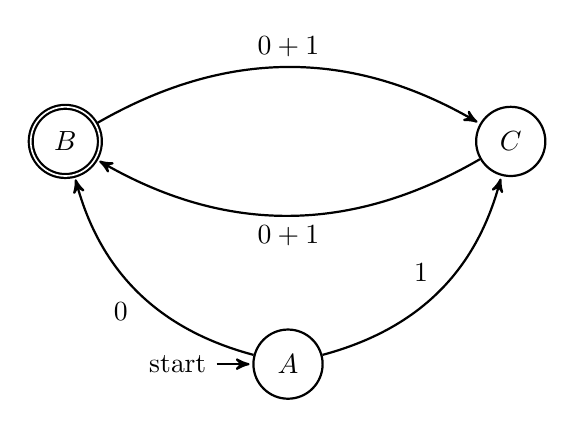
\begin{tikzpicture}
	[->,>=stealth',shorten >=1pt,auto,node distance=4cm,
		thick,base node/.style={circle,draw,minimum size=16pt}, real node/.style={double,circle,draw,minimum size=35pt}]

	\node[accepting, state]    (B)       {$B$};
	\node[initial, initial text={start}, state] [below right of=B] (A) {$A$};
	\node[state]    (C)     [above right of = A]  {$C$};

	\path[]
	(A) edge [bend left]   node {$0$}  (B)
	(A) edge [bend right]   node {$1$}  (C)
	(B) edge [bend left]   node {$0+1$}  (C)
	(C) edge [bend left]   node {$0+1$}  (B)

	;

\end{tikzpicture}\\

Delete C, we get:\\

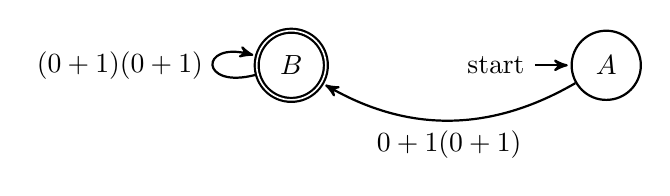
\begin{tikzpicture}
	[->,>=stealth',shorten >=1pt,auto,node distance=4cm,
		thick,base node/.style={circle,draw,minimum size=16pt}, real node/.style={double,circle,draw,minimum size=35pt}]

	\node[accepting, state]    (B)       {$B$};
	\node[initial, initial text={start}, state] [right of=B] (A) {$A$};
	% \node[state]    (C)     [above right of = A]  {$C$};

	\path[]
	(A) edge [bend left]   node {$0+1(0+1)$}  (B)
	% (A) edge [bend right]   node {$1$}  (C)
	% (B) edge [bend left]   node {$0+1$}  (C)
	(B) edge [loop left]   node {$(0+1)(0+1)$}  (B)

	;

\end{tikzpicture}\\

And the answer will be $(0+1(0+1))(0+1)^* $


\subsection{d}

First, let's construct two automata, noted as M1 and M2.\\

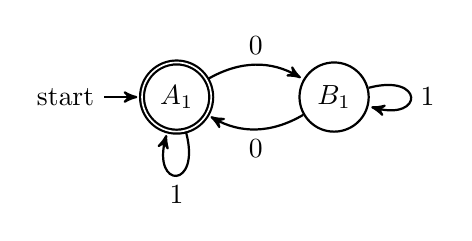
\begin{tikzpicture}
	[->,>=stealth',shorten >=1pt,auto,node distance=2cm,
		thick,base node/.style={circle,draw,minimum size=16pt}, real node/.style={double,circle,draw,minimum size=35pt}]

	\node[initial, initial text={start},accepting, state]  (A1) {$A_1$};
	\node[state]  [right of=A1]  (B1)       {$B_1$};
	% \node[state]    (C)     [above right of = A]  {$C$};

	\path[]
	(A1) edge [bend left]   node {$0$}  (B1)
	(A1) edge [loop below]   node {$1$}  (A1)
	(B1) edge [bend left]   node {$0$}  (A1)
	(B1) edge [loop right]   node {$1$}  (B1)
	% (A) edge [bend right]   node {$1$}  (C)
	% (B) edge [bend left]   node {$0+1$}  (C)
	% (B) edge [loop left]   node {$(0+1)(0+1)$}  (B)

	;

\end{tikzpicture}\\

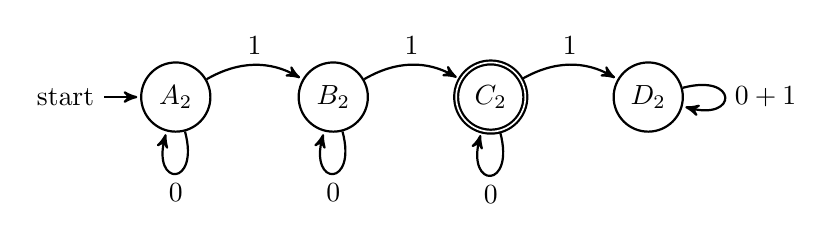
\begin{tikzpicture}
	[->,>=stealth',shorten >=1pt,auto,node distance=2cm,
		thick,base node/.style={circle,draw,minimum size=16pt}, real node/.style={double,circle,draw,minimum size=35pt}]

	\node[initial, initial text={start}, state]  (A2) {$A_2$};
	\node[state]  [right of=A2]  (B2)       {$B_2$};
	\node[state,accepting]  [right of=B2]  (C2)       {$C_2$};
	\node[state]  [right of=C2]  (D2)       {$D_2$};
	% \node[state]    (C)     [above right of = A]  {$C$};

	\path[]
	(A2) edge [bend left]   node {$1$}  (B2)
	(A2) edge [loop below]   node {$0$}  (A2)
	(B2) edge [loop below]   node {$0$}  (B2)
	(C2) edge [loop below]   node {$0$}  (C2)
	(B2) edge [bend left]   node {$1$}  (C2)
	(C2) edge [bend left]   node {$1$}  (D2)
	(D2) edge [loop right]   node {$0+1$}  (D2)

	;

\end{tikzpicture}\\

Then we make the product of M1 and M2.\\

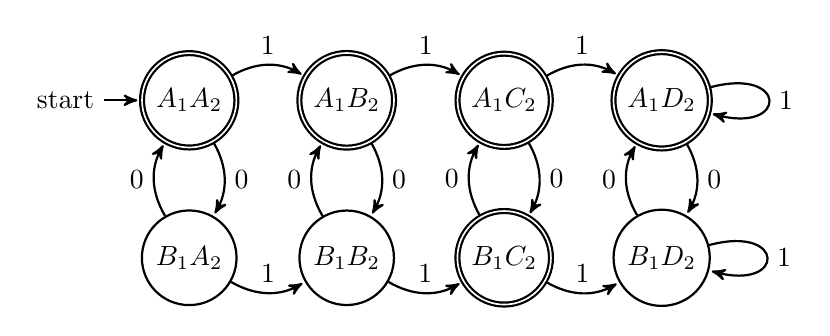
\begin{tikzpicture}
	[->,>=stealth',shorten >=1pt,auto,node distance=2cm,
		thick,base node/.style={circle,draw,minimum size=16pt}, real node/.style={double,circle,draw,minimum size=35pt}]

	\node[accepting, initial, initial text={start}, state]  (A) {$A_1A_2$};
	\node[accepting,state]  [right of=A]  (B)       {$A_1B_2$};
	\node[accepting,state]  [right of=B]  (C)       {$A_1C_2$};
	\node[accepting,state]  [right of=C]  (D)       {$A_1D_2$};
	\node[state]  [below of=A]  (E)       {$B_1A_2$};
	\node[state]  [right of=E]  (F)       {$B_1B_2$};
	\node[accepting,state]  [right of=F]  (G)       {$B_1C_2$};
	\node[state]  [right of=G]  (H)       {$B_1D_2$};
	% \node[state]    (C)     [above right of = A]  {$C$};

	\path[]
	(A) edge [bend left]   node {$1$}  (B)
	(B) edge [bend left]   node {$1$}  (C)
	(C) edge [bend left]   node {$1$}  (D)

	(E) edge [bend right]   node {$1$}  (F)
	(F) edge [bend right]   node {$1$}  (G)
	(G) edge [bend right]   node {$1$}  (H)

	(D) edge [loop right]   node {$1$}  (D)
	(H) edge [loop right]   node {$1$}  (H)

	(A) edge [bend left]   node {$0$}  (E)
	(E) edge [bend left]   node {$0$}  (A)
	(B) edge [bend left]   node {$0$}  (F)
	(F) edge [bend left]   node {$0$}  (B)
	(C) edge [bend left]   node {$0$}  (G)
	(G) edge [bend left]   node {$0$}  (C)
	(D) edge [bend left]   node {$0$}  (H)
	(H) edge [bend left]   node {$0$}  (D)
	;

\end{tikzpicture}\\

Then we rename it as follows:\\

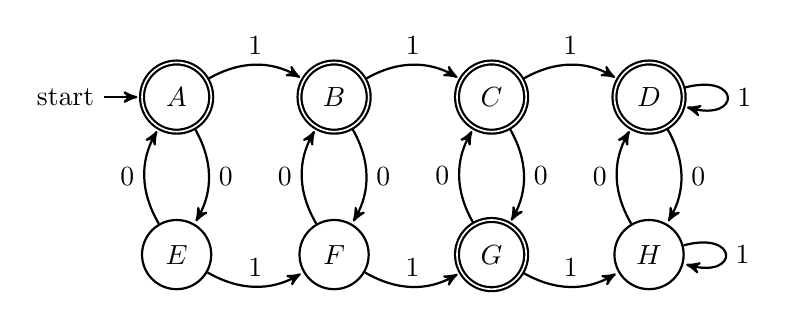
\begin{tikzpicture}
	[->,>=stealth',shorten >=1pt,auto,node distance=2cm,
		thick,base node/.style={circle,draw,minimum size=16pt}, real node/.style={double,circle,draw,minimum size=35pt}]

	\node[accepting, initial, initial text={start}, state]  (A) {$A$};
	\node[accepting,state]  [right of=A]  (B)       {$B$};
	\node[accepting,state]  [right of=B]  (C)       {$C$};
	\node[accepting,state]  [right of=C]  (D)       {$D$};
	\node[state]  [below of=A]  (E)       {$E$};
	\node[state]  [right of=E]  (F)       {$F$};
	\node[accepting,state]  [right of=F]  (G)       {$G$};
	\node[state]  [right of=G]  (H)       {$H$};
	% \node[state]    (C)     [above right of = A]  {$C$};

	\path[]
	(A) edge [bend left]   node {$1$}  (B)
	(B) edge [bend left]   node {$1$}  (C)
	(C) edge [bend left]   node {$1$}  (D)

	(E) edge [bend right]   node {$1$}  (F)
	(F) edge [bend right]   node {$1$}  (G)
	(G) edge [bend right]   node {$1$}  (H)

	(D) edge [loop right]   node {$1$}  (D)
	(H) edge [loop right]   node {$1$}  (H)

	(A) edge [bend left]   node {$0$}  (E)
	(E) edge [bend left]   node {$0$}  (A)
	(B) edge [bend left]   node {$0$}  (F)
	(F) edge [bend left]   node {$0$}  (B)
	(C) edge [bend left]   node {$0$}  (G)
	(G) edge [bend left]   node {$0$}  (C)
	(D) edge [bend left]   node {$0$}  (H)
	(H) edge [bend left]   node {$0$}  (D)
	;

\end{tikzpicture}\\

Delete F, \\

\begin{tikzpicture}
	[->,>=stealth',shorten >=1pt,auto,node distance=2cm,
		thick,base node/.style={circle,draw,minimum size=16pt}, real node/.style={double,circle,draw,minimum size=35pt}]

	\node[accepting, initial, initial text={start}, state]  (A) {$A$};
	\node[accepting,state]  [right of=A]  (B)       {$B$};
	\node[accepting,state]  [right of=B]  (C)       {$C$};
	\node[accepting,state]  [right of=C]  (D)       {$D$};
	\node[state]  [below of=A]  (E)       {$E$};
	% \node[state]  [right of=E]  (F)       {$F$};
	\node[accepting,state]  [right of=F]  (G)       {$G$};
	\node[state]  [right of=G]  (H)       {$H$};
	% \node[state]    (C)     [above right of = A]  {$C$};

	\path[]
	(A) edge [bend left]   node {$1$}  (B)
	(B) edge [bend left]   node {$1$}  (C)
	(C) edge [bend left]   node {$1$}  (D)

	(E) edge [bend right]   node {$10$}  (B)
	(E) edge [bend right]   node {$11$}  (G)
	(B) edge [bend right]   node {$01$}  (G)
	(G) edge [bend right]   node {$1$}  (H)

	(D) edge [loop right]   node {$1$}  (D)
	(H) edge [loop right]   node {$1$}  (H)

	(A) edge [bend left]   node {$0$}  (E)
	(E) edge [bend left]   node {$0$}  (A)
	(B) edge [loop above]   node {$00$}  (B)
	% (F) edge [bend left]   node {$0$}  (B)
	(C) edge [bend left]   node {$0$}  (G)
	(G) edge [bend left]   node {$0$}  (C)
	(D) edge [bend left]   node {$0$}  (H)
	(H) edge [bend left]   node {$0$}  (D)
	;

\end{tikzpicture}\\

Delete E,\\

\begin{tikzpicture}
	[->,>=stealth',shorten >=1pt,auto,node distance=2cm,
		thick,base node/.style={circle,draw,minimum size=16pt}, real node/.style={double,circle,draw,minimum size=35pt}]

	\node[accepting, initial, initial text={start}, state]  (A) {$A$};
	\node[accepting,state]  [right of=A]  (B)       {$B$};
	\node[accepting,state]  [right of=B]  (C)       {$C$};
	\node[accepting,state]  [right of=C]  (D)       {$D$};
	% \node[state]  [below of=A]  (E)       {$E$};
	% \node[state]  [right of=E]  (F)       {$F$};
	\node[accepting,state]  [right of=F]  (G)       {$G$};
	\node[state]  [right of=G]  (H)       {$H$};
	% \node[state]    (C)     [above right of = A]  {$C$};

	\path[]
	(A) edge [bend left]   node {$1+010$}  (B)
	(A) edge [loop below]   node {$00$}  (A)
	(B) edge [loop above]   node {$00$}  (B)
	(B) edge [bend left]   node {$1$}  (C)
	(C) edge [bend left]   node {$1$}  (D)

	(A) edge [bend right]   node {$011$}  (G)
	(B) edge [bend right]   node {$01$}  (G)
	(G) edge [bend right]   node {$1$}  (H)

	(D) edge [loop right]   node {$1$}  (D)
	(H) edge [loop right]   node {$1$}  (H)


	% (B) edge [loop above]   node {$00$}  (B)
	% (F) edge [bend left]   node {$0$}  (B)
	(C) edge [bend left]   node {$0$}  (G)
	(G) edge [bend left]   node {$0$}  (C)
	(D) edge [bend left]   node {$0$}  (H)
	(H) edge [bend left]   node {$0$}  (D)
	;

\end{tikzpicture}\\

Delete H,\\

\begin{tikzpicture}
	[->,>=stealth',shorten >=1pt,auto,node distance=3cm,
		thick,base node/.style={circle,draw,minimum size=16pt}, real node/.style={double,circle,draw,minimum size=35pt}]

	\node[accepting, initial, initial text={start}, state]  (A) {$A$};
	\node[accepting,state]  [right of=A]  (B)       {$B$};
	\node[accepting,state]  [right of=B]  (C)       {$C$};
	\node[accepting,state]  [right of=C]  (D)       {$D$};
	% \node[state]  [below of=A]  (E)       {$E$};
	% \node[state]  [right of=E]  (F)       {$F$};
	\node[accepting,state]  [right of=F]  (G)       {$G$};
	% \node[state]  [right of=G]  (H)       {$H$};
	% \node[state]    (C)     [above right of = A]  {$C$};

	\path[]
	(A) edge [bend left]   node {$1+010$}  (B)
	(A) edge [loop below]   node {$00$}  (A)
	(B) edge [loop above]   node {$00$}  (B)
	(B) edge [bend left]   node {$1$}  (C)
	(C) edge [bend left]   node {$1$}  (D)

	(A) edge [bend right]   node {$011$}  (G)
	(B) edge [bend right]   node {$01$}  (G)
	% (G) edge [bend right]   node {$1$}  (H)

	(D) edge [loop right]   node {$1+01^*0$}  (D)
	% (H) edge [loop right]   node {$1$}  (H)


	% (B) edge [loop above]   node {$00$}  (B)
	% (F) edge [bend left]   node {$0$}  (B)
	(C) edge [bend left]   node {$0$}  (G)
	(G) edge [bend left]   node {$0$}  (C)
	(G) edge [bend right]   node {$11^*0$}  (D)
	% (D) edge [bend left]   node {$0$}  (H)
	% (H) edge [bend left]   node {$0$}  (D)
	;

\end{tikzpicture}\\
\textbf{Case1}: choose A as accepting state. We can get $(00)^*$\\
\textbf{Case2}: choose B as accepting state. We can get $(00)^*(1+010)(00)^*$\\
\textbf{Case3}: choose C as accepting state. We can get \\
Where \[L_1=011+(1+010)(00)^*01\]
\[L_2=(1+010)(00)^*1\]
\begin{tikzpicture}
	[->,>=stealth',shorten >=1pt,auto,node distance=3cm,
		thick,base node/.style={circle,draw,minimum size=16pt}, real node/.style={double,circle,draw,minimum size=35pt}]

	\node[accepting, initial, initial text={start}, state]  (A) {$A$};
	% \node[accepting,state]  [right of=A]  (B)       {$B$};
	\node[accepting,state]  [right of=B]  (C)       {$C$};
	\node[accepting,state]  [right of=C]  (D)       {$D$};
	% \node[state]  [below of=A]  (E)       {$E$};
	% \node[state]  [right of=E]  (F)       {$F$};
	% \node[accepting,state]  [right of=F]  (G)       {$G$};
	% \node[state]  [right of=G]  (H)       {$H$};
	% \node[state]    (C)     [above right of = A]  {$C$};

	\path[]
	% (A) edge [bend left]   node {$1+010$}  (B)
	(A) edge [loop below]   node {$00$}  (A)
	% (B) edge [loop above]   node {$00$}  (B)
	(A) edge   node {$L_2+L_10$}  (C)
	(C) edge [loop above]   node {$(00)^*$}  (C)
	(C) edge  node {$1+011^*0$}  (D)

	(A) edge [bend right]   node {$L_111^*0$}  (D)
	% (B) edge [bend right]   node {$01$}  (G)
	% (G) edge [bend right]   node {$1$}  (H)

	(D) edge [loop right]   node {$1+01^*0$}  (D)
	% (H) edge [loop right]   node {$1$}  (H)


	% (B) edge [loop above]   node {$00$}  (B)
	% (F) edge [bend left]   node {$0$}  (B)
	% (C) edge [bend left]   node {$0$}  (G)
	% (G) edge [bend left]   node {$0$}  (C)
	% (G) edge [bend right]   node {$11^*0$}  (D)
	% (D) edge [bend left]   node {$0$}  (H)
	% (H) edge [bend left]   node {$0$}  (D)
	;

\end{tikzpicture}\\
Then we can get $(00)^*(L_2+L_10)(00)^*$\\
\textbf{Case4}: choose D as accepting state. We can get $(00)^*(L_21+(L_1+L_20)(00)^*(11^*0+01))(1+01^*0)^* $\\
\textbf{Case5}: choose G as accepting state. We can get:\\

\begin{tikzpicture}
	[->,>=stealth',shorten >=1pt,auto,node distance=3cm,
		thick,base node/.style={circle,draw,minimum size=16pt}, real node/.style={double,circle,draw,minimum size=35pt}]

	\node[accepting, initial, initial text={start}, state]  (A) {$A$};
	% \node[accepting,state]  [right of=A]  (B)       {$B$};
	% \node[accepting,state]  [right of=B]  (C)       {$C$};
	\node[accepting,state]  [right of=C]  (D)       {$D$};
	% \node[state]  [below of=A]  (E)       {$E$};
	% \node[state]  [right of=E]  (F)       {$F$};
	\node[accepting,state]  [right of=F]  (G)       {$G$};
	% \node[state]  [right of=G]  (H)       {$H$};
	% \node[state]    (C)     [above right of = A]  {$C$};

	\path[]
	% (A) edge [bend left]   node {$1+010$}  (B)
	(A) edge [loop below]   node {$00$}  (A)
	% (B) edge [loop above]   node {$00$}  (B)
	(A) edge   node {$L_20+L_1$}  (G)
	(G) edge [loop below]   node {$(00)^*$}  (G)
	(G) edge  node {$11^*0+01$}  (D)

	(A) edge   node {$L_21$}  (D)
	% (B) edge [bend right]   node {$01$}  (G)
	% (G) edge [bend right]   node {$1$}  (H)

	(D) edge [loop right]   node {$1+01^*0$}  (D)
	% (H) edge [loop right]   node {$1$}  (H)


	% (B) edge [loop above]   node {$00$}  (B)
	% (F) edge [bend left]   node {$0$}  (B)
	% (C) edge [bend left]   node {$0$}  (G)
	% (G) edge [bend left]   node {$0$}  (C)
	% (G) edge [bend right]   node {$11^*0$}  (D)
	% (D) edge [bend left]   node {$0$}  (H)
	% (H) edge [bend left]   node {$0$}  (D)
	;

\end{tikzpicture}\\
Then we can get $(00)^*(L_1+L_20)(00)^* $\\

In all, the answer should be $(00)^* + (00)^*(1+010)(00)^* + (00)^*(L_2+L_10)(00)^*
	+(00)^*(L_21+(L_1+L_20)(00)^*(11^*0+01))(1+01^*0)^* + (00)^*(L_1+L_20)(00)^* $

\subsection{e}

\begin{tikzpicture}
	[->,>=stealth',shorten >=1pt,auto,node distance=2cm,
		thick,base node/.style={circle,draw,minimum size=16pt}, real node/.style={double,circle,draw,minimum size=35pt}]

	\node[accepting, initial, initial text={start}, state]  (A) {$A$};
	\node[accepting,state]  [right of=A]  (B)       {$B$};
	\node[accepting,state]  [right of=B]  (C)       {$C$};
	\node[accepting,state]  [right of=C]  (D)       {$D$};
	% \node[state]  [below of=A]  (E)       {$E$};
	% \node[state]  [right of=E]  (F)       {$F$};
	\node[state]  [right of=F]  (F)       {$F$};
	% \node[state]  [right of=G]  (H)       {$H$};
	% \node[state]    (C)     [above right of = A]  {$C$};

	\path[]
	(A) edge [bend left]   node {$1$}  (B)
	(B) edge [bend left]   node {$0$}  (A)
	% (A) edge [loop below]   node {$00$}  (A)
	% (B) edge [loop above]   node {$00$}  (B)
	(B) edge [bend left]   node {$1$}  (C)
	(C) edge [bend left]   node {$0$}  (D)
	(D) edge [bend left]   node {$1$}  (C)
	(C) edge [bend left]   node {$1$}  (F)

	(A) edge [loop below]   node {$0$}  (A)
	(D) edge [loop right]   node {$0$}  (D)

	(F) edge [loop right]   node {$1+0$}  (F)
	;

\end{tikzpicture}\\
\textbf{Case1}: Choose A as the accepting state. Then we get $(0+10)^* $\\
\textbf{Case2}: Choose B as the accepting state. Then we get $(0+10)^*1 $\\
\textbf{Case3}: Choose C as the accepting state. Then we get $(0+10)^*11(00^*1)^* $\\
\textbf{Case4}: Choose D as the accepting state. Then we get $(0+10)^*110(0+10)^* $\\

Finally, the answer should be $(0+10)^* + (0+10)^*1 + (0+10)^*11(00^*1)^* + (0+10)^*110(0+10)^* $


\section{PROBLEM 2}
First, construct the $\epsilon-NFA$ as follows.\\
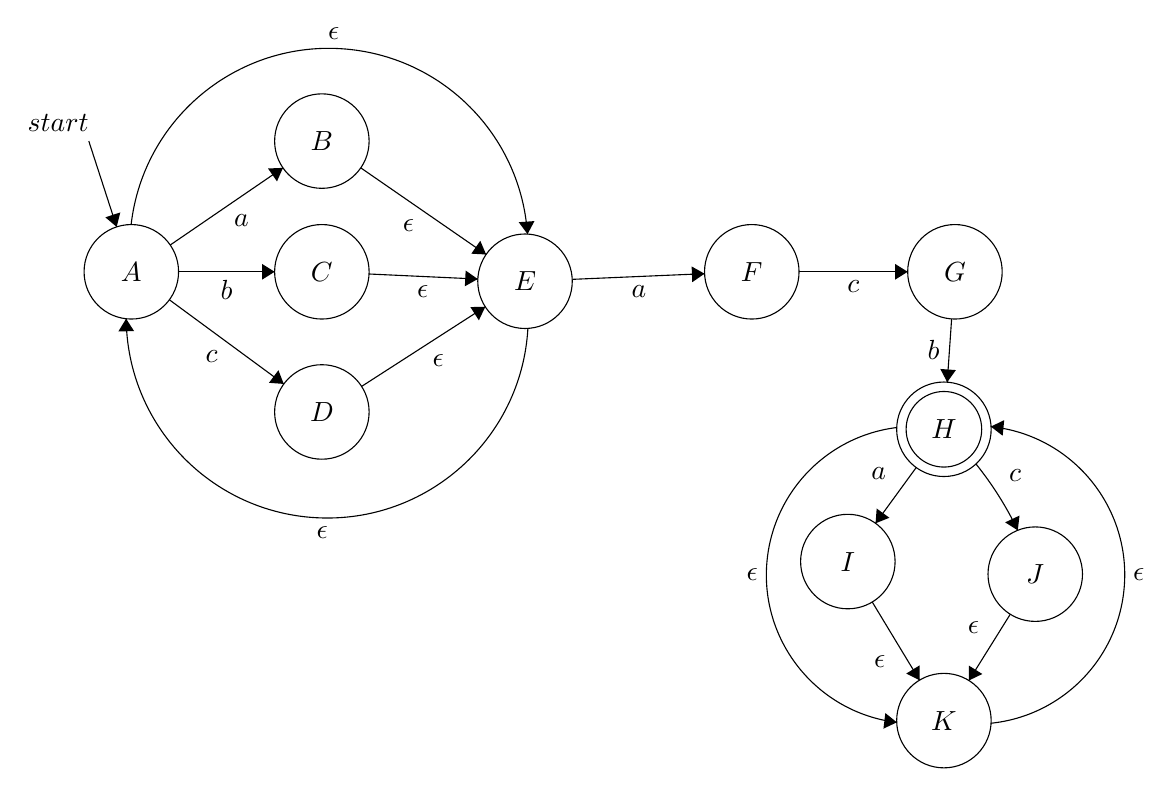
\begin{tikzpicture}[scale=0.2]
	\tikzstyle{every node}+=[inner sep=0pt]
	\draw [black] (8.2,-18.2) circle (3);
	\draw (8.2,-18.2) node {$A$};
	\draw [black] (20.3,-9.9) circle (3);
	\draw (20.3,-9.9) node {$B$};
	\draw [black] (20.3,-18.2) circle (3);
	\draw (20.3,-18.2) node {$C$};
	\draw [black] (20.3,-27.1) circle (3);
	\draw (20.3,-27.1) node {$D$};
	\draw [black] (33.2,-18.8) circle (3);
	\draw (33.2,-18.8) node {$E$};
	\draw [black] (47.6,-18.2) circle (3);
	\draw (47.6,-18.2) node {$F$};
	\draw [black] (60.5,-18.2) circle (3);
	\draw (60.5,-18.2) node {$G$};
	\draw [black] (59.8,-28.2) circle (3);
	\draw (59.8,-28.2) node {$H$};
	\draw [black] (59.8,-28.2) circle (2.4);
	\draw [black] (53.7,-36.6) circle (3);
	\draw (53.7,-36.6) node {$I$};
	\draw [black] (65.6,-37.4) circle (3);
	\draw (65.6,-37.4) node {$J$};
	\draw [black] (59.8,-46.7) circle (3);
	\draw (59.8,-46.7) node {$K$};
	\draw [black] (10.67,-16.5) -- (17.83,-11.6);
	\fill [black] (17.83,-11.6) -- (16.88,-11.64) -- (17.45,-12.46);
	\draw (15.2,-14.55) node [below] {$a$};
	\draw [black] (11.2,-18.2) -- (17.3,-18.2);
	\fill [black] (17.3,-18.2) -- (16.5,-17.7) -- (16.5,-18.7);
	\draw (14.25,-18.7) node [below] {$b$};
	\draw [black] (10.62,-19.98) -- (17.88,-25.32);
	\fill [black] (17.88,-25.32) -- (17.54,-24.45) -- (16.94,-25.25);
	\draw (13.3,-23.15) node [below] {$c$};
	\draw [black] (33.383,-21.787) arc (-3.21772:-179.53195:12.765);
	\fill [black] (7.87,-21.18) -- (7.38,-21.98) -- (8.38,-21.97);
	\draw (20.32,-34.35) node [below] {$\epsilon$};
	\draw [black] (8.187,-15.207) arc (-186.55153:-356.19814:12.64);
	\fill [black] (33.36,-15.81) -- (33.8,-14.98) -- (32.8,-15.05);
	\draw (21.06,-3.49) node [above] {$\epsilon$};
	\draw [black] (22.77,-11.6) -- (30.73,-17.1);
	\fill [black] (30.73,-17.1) -- (30.36,-16.23) -- (29.79,-17.05);
	\draw (25.8,-14.85) node [below] {$\epsilon$};
	\draw [black] (23.3,-18.34) -- (30.2,-18.66);
	\fill [black] (30.2,-18.66) -- (29.43,-18.12) -- (29.38,-19.12);
	\draw (26.71,-19.04) node [below] {$\epsilon$};
	\draw [black] (22.82,-25.48) -- (30.68,-20.42);
	\fill [black] (30.68,-20.42) -- (29.73,-20.44) -- (30.27,-21.28);
	\draw (27.69,-23.45) node [below] {$\epsilon$};
	\draw [black] (36.2,-18.68) -- (44.6,-18.32);
	\fill [black] (44.6,-18.32) -- (43.78,-17.86) -- (43.82,-18.86);
	\draw (40.43,-19.04) node [below] {$a$};
	\draw [black] (50.6,-18.2) -- (57.5,-18.2);
	\fill [black] (57.5,-18.2) -- (56.7,-17.7) -- (56.7,-18.7);
	\draw (54.05,-18.7) node [below] {$c$};
	\draw [black] (60.29,-21.19) -- (60.01,-25.21);
	\fill [black] (60.01,-25.21) -- (60.56,-24.44) -- (59.57,-24.37);
	\draw (59.55,-23.16) node [left] {$b$};
	\draw [black] (58.04,-30.63) -- (55.46,-34.17);
	\fill [black] (55.46,-34.17) -- (56.34,-33.82) -- (55.53,-33.23);
	\draw (56.16,-31.02) node [left] {$a$};
	\draw [black] (61.835,-30.401) arc (38.79886:25.65866:21.767);
	\fill [black] (64.49,-34.62) -- (64.6,-33.68) -- (63.69,-34.11);
	\draw (63.91,-31.13) node [right] {$c$};
	\draw [black] (55.25,-39.17) -- (58.25,-44.13);
	\fill [black] (58.25,-44.13) -- (58.26,-43.19) -- (57.41,-43.71);
	\draw (56.11,-42.92) node [left] {$\epsilon$};
	\draw [black] (64.01,-39.95) -- (61.39,-44.15);
	\fill [black] (61.39,-44.15) -- (62.24,-43.74) -- (61.39,-43.21);
	\draw (62.07,-40.76) node [left] {$\epsilon$};
	\draw [black] (62.783,-28.033) arc (84.12878:-84.12878:9.467);
	\fill [black] (62.78,-28.03) -- (63.53,-28.61) -- (63.63,-27.62);
	\draw (71.78,-37.45) node [right] {$\epsilon$};
	\draw [black] (56.815,-46.813) arc (-96.95379:-263.04621:9.432);
	\fill [black] (56.81,-46.81) -- (56.08,-46.22) -- (55.96,-47.21);
	\draw (48.02,-37.45) node [left] {$\epsilon$};
	\draw [black] (5.5,-9.9) -- (7.27,-15.35);
	\draw (3.55,-9.31) node [above] {$start$};
	\fill [black] (7.27,-15.35) -- (7.5,-14.43) -- (6.55,-14.74);
\end{tikzpicture}
Then we can generate the DFA from the start state.\\

\begin{tabular}{cccc}
	     & a    & b   & c   \\
	->AE & ABEF & ACE & ADE
\end{tabular}\\

Also, we add all the new state appearing at the 'a' 'b' 'c' columns.

\begin{tabular}{cccc}
	     & a    & b   & c    \\
	->AE & ABEF & ACE & ADE  \\
	ABEF & ABEF & ACE & ADEG \\
\end{tabular}\\
Then repeat this process until no new state appears. Finally, we get:\\
\begin{tabular}{llll}
	         & a       & b     & c       \\
	->AE     & ABEF    & ACE   & ADE     \\
	ABEF     & ABEF    & ACE   & ADEG    \\
	ACE      & ABEF    & ACE   & ADE     \\
	ADE      & ABEF    & ACE   & ADE     \\
	ADEG     & ABEF    & ACEHK & ADE     \\
	*ACEHK   & ABEFHIK & ACE   & ADEHJK  \\
	*ABEFHIK & ABEFHIK & ACE   & ADEGHJK \\
	*ADEHJK  & ABEFHIK & ACE   & ADEHJK  \\
	*ADEGHJK & ABEFHIK & ACEHK & ADEHJK  \\
\end{tabular}\\

\section{PROBLEM 3}
First, let's prove that $(L+M)^*=(L^*M^*)^*$.\\

$(L+M)^*\subseteq(L^*M^*)^*$:\\
$\forall s:string \in (L+M)^*, suppose\ that\ s \ne \epsilon.$
Then $s$ can be written as $w_1w_2w_3...$, where $w_i \in (L+M)$.
If $w_i \in L$, then $w_i \in L^*M^*$.
Also, if $w_i \in M$, then $w_i \in L^*M^*$, so $s \in (L^*M^*)^*$.\\
$(L^*M^*)^*\subseteq(L+M)^*$:\\
$\forall t:string \in (L^*M^*)^*, suppose\ that\ t \ne \epsilon.$
Then t can be written as $u_1u_2u_3...$, where $u_i \in L^*M^*$.
Then $u_i$ can be written as $l_1l_2....m_1m_2...$, where $l_i \in L\ or\ l_i=\epsilon$;
$m_i \in M \ or\ m_i=\epsilon$. Then $l_i \in (L+M)$ and $m_i \in (L+M)$.
So $u_i \in (L+M)^*$, so $t \in (L+M)^*$. \\
If $s$ or $t$ is $\epsilon$, it's obvious that both of them are in both set.

Given that $L_1+L_2+L_3=L_1+(L_2+L_3)\ ,(L^*)^*=L\ and\ L_1L_2L_3=L_1(L_2L_3) $, we can get:\\
\begin{alignat*}{2}
	(L_1+L_2+L_3+L_4)^* & =(L_1+(L_2+L_3+L_4))^*                \\
	                    & =(L_1^*(L_2+L_3+L_4)^*)^*             \\
	                    & =(L_1^*(L_2+(L_3+L_4))^*)^*           \\
	                    & =(L_1^*(L_2^*(L_3+L_4)^*)^*)^*        \\
	                    & =(L_1^*(L_2^*((L_3^*L_4^*)^*)^*)^*)^* \\
	                    & =(L_1^*L_2^*L_3^*L_4^*)^*
\end{alignat*}

\section{PROBLEM 4}
\subsection{a}
\[R_{11}^0 = \epsilon\ R_{12}^0=a\ R_{13}^0=\emptyset\]
\[R_{21}^0 = d\ R_{22}^0=\epsilon+e\ R_{23}^0=b\]
\[R_{31}^0 = \emptyset\ R_{32}^0=c\ R_{33}^0=\epsilon\]
\subsection{b}
\[R_{11}^1 = R_{11}^0 +R_{11}^0R_{11}^{0*}R_{11}^0 = \epsilon  \]
\[R_{12}^1 = R_{12}^0 +R_{11}^0R_{11}^{0*}R_{12}^0 = a  \]
\[R_{13}^1 = R_{13}^0 +R_{11}^0R_{11}^{0*}R_{13}^0 = \emptyset  \]

\[R_{21}^1 = R_{21}^0 +R_{21}^0R_{11}^{0*}R_{11}^0 = d  \]
\[R_{22}^1 = R_{22}^0 +R_{21}^0R_{11}^{0*}R_{12}^0 = \epsilon+e+da  \]
\[R_{23}^1 = R_{23}^0 +R_{21}^0R_{11}^{0*}R_{13}^0 = b  \]

\[R_{31}^1 = R_{31}^0 +R_{31}^0R_{11}^{0*}R_{11}^0 = \emptyset  \]
\[R_{32}^1 = R_{32}^0 +R_{31}^0R_{11}^{0*}R_{12}^0 = c  \]
\[R_{33}^1 = R_{33}^0 +R_{31}^0R_{11}^{0*}R_{13}^0 = \epsilon  \]

\subsection{c}
\[R_{11}^2 = R_{11}^1 +R_{12}^1R_{22}^{1*}R_{21}^1 = \epsilon+a(da+e)^*d  \]
\[R_{12}^2 = R_{12}^1 +R_{12}^1R_{22}^{1*}R_{22}^1 = a+a(da+e)^*=a(da+e)^*  \]
\[R_{13}^2 = R_{13}^1 +R_{12}^1R_{22}^{1*}R_{23}^1 = a(da+e)^*b  \]

\[R_{21}^2 = R_{21}^1 +R_{22}^1R_{22}^{1*}R_{21}^1 = d+(da+e)^*d=(da+e)^*d  \]
\[R_{22}^2 = R_{22}^1 +R_{22}^1R_{22}^{1*}R_{22}^1 = (\epsilon+e+da)+(e+da)^*=(e+da)^*  \]
\[R_{23}^2 = R_{23}^1 +R_{22}^1R_{22}^{1*}R_{23}^1 = b+(e+da)^*b=(e+da)^*b  \]

\[R_{31}^2 = R_{31}^1 +R_{32}^1R_{22}^{1*}R_{21}^1 = c(e+da)^*d  \]
\[R_{32}^2 = R_{32}^1 +R_{32}^1R_{22}^{1*}R_{22}^1 = c+c(e+da)^*=c(e+da)^*  \]
\[R_{33}^2 = R_{33}^1 +R_{32}^1R_{22}^{1*}R_{23}^1 = \epsilon+c(e+da)^*b  \]

\subsection{d}
\begin{alignat*}{2}
	R_{13}^3 & =R_{13}^2+R_{13}^2R_{33}^{2*}R_{33}^2                                \\
	         & =a(da+e)^*b+(a(da+e)^*b)(\epsilon+c(e+da)^*b)^*(\epsilon+c(e+da)^*b) \\
	         & =a(da+e)^*b(\epsilon+(c(e+da)^*b)^*)                                 \\
	         & =a(da+e)^*b(c(e+da)^*b)^*
\end{alignat*}

\section{PROBLEM 5}

Define the automata of $B^R$ as follows.

\begin{alignat*}{2}
	Q      & ={Carry,Clear}                                             \\
	q_0    & =Clear                                                     \\
	\Sigma & = \Sigma_3                                                 \\
	\delta & = \{\delta(Clear,p)=Clear|p\in\{(101),(010),(000)\}\}      \\
	       & \cup \{\delta(Clear,p)=Carry|p\in\{(110)\} \}              \\
	       & \cup \{\delta(Carry,p)=Carry|p\in\{(111),(100),(010) \} \} \\
	       & \cup \{\delta(Carry,p)=Clear|p\in\{(001) \} \}             \\
	F      & =Clear
\end{alignat*}\\

Intuitively, we can draw the automata as follows:\\

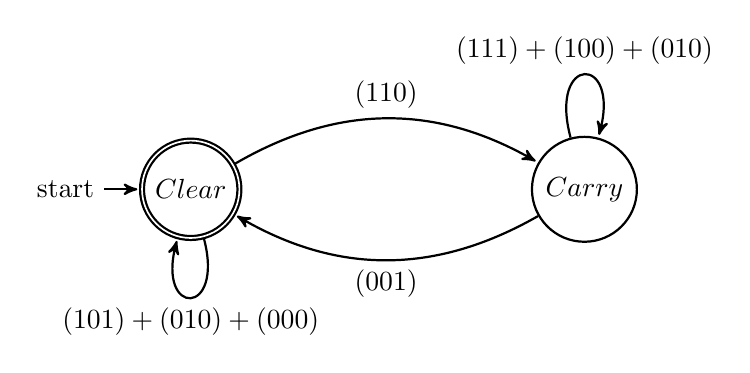
\begin{tikzpicture}
	[->,>=stealth',shorten >=1pt,auto,node distance=5cm,
		thick,base node/.style={circle,draw,minimum size=16pt}, real node/.style={double,circle,draw,minimum size=35pt}]

	\node[accepting, initial, initial text={start}, state]  (A) {$Clear$};
	\node[state]  [right of=A]  (B)       {$Carry$};

	\path[]
	(A) edge [bend left]   node {$(110)$}  (B)
	(B) edge [bend left]   node {$(001)$}  (A)
	% (A) edge [loop below]   node {$00$}  (A)
	(B) edge [loop above]   node {$(111)+(100)+(010) $}  (B)
	(A) edge [loop below]   node {$(101)+(010)+(000) $}  (A)
	;

\end{tikzpicture}\\

So $B^R$ is regular, then $B$ is regular.

\section{PROBLEM 6}
\subsection{a}
$\forall n \in N^* $, we can found string $ww$ such that $|w|>n$.
Now let's write $w$ as $uv$ where $|u|=n$. So for any division of
$w$, $xy$ is a substring of $u$ since $|xy|<n$.\\
Just make sure that we choose a string where $v$ is not a substring of $u$.\\
Then it's impossible to represent $v$ as $y^k$.\\
But $v$ is a substring of $z$, so $z$ cannot be written as $y^k$.\\
Finally, we can get the conclusion that $xy^kz$ cannot be
written as $ww$ for all the $k$. (Just choose $k$ such that
$k|y|>|z|$, if $xy^kz$ can be written as $ww$, then $z$ is a substring of $y$,
which is in contrast to our hypothesis.)

\subsection{b}
$\forall k \in N^* $ , choose a string $s$ where $n>k$, so $y$ contains at least one
$0$. In such case, $xy^0z=xz$ is obvious not contained in the set since the number
of $0$ is less than the number of $2$.

\subsection{c}
$\forall n \in N^*$, let $i$ be a prime which is larger than $n+2$, let $j$ be $(i-1)!$.\\
$gcd(i,j)=1$ since $i$ is a prime.\\
Because $|xy|<n$, $y$ contains only $0$. So the number of $0$ in $xy^0z$ is less than
$i$ since $y \ne \epsilon$. Also, $i$ is larger than $n+2$, so the number of $0$ in $xz$ is larger
than $2$.\\
So $gcd(the\ number\ of\ 0\ in\ xz, j) \geq 2$, which means $xy^0z$ is not in the set.

\subsection{d}
$\forall n \in N^* $, let $x_1=1^n$, $x_i=1^{n+i}, i\in [2,n]$\\
Since $|xy|\leq n$, so $y$ only contains $1$. So the number of $1$ in $x_1$ in $xy^2z$
range from $n+1$ to $n+n$, which must be equal to some $x_i$. Then $xy^2z$ is not
in the set.

\section{PROBLEM 7}
Suppose that the alphabet of $A$ and $B$ is $\Sigma$. A string $w$ that contains
strings in $B$ as substring can be written as $(\Sigma^*B\Sigma^*)^+$.\\
Given that $A$ and $B$ are regular. Then $(\Sigma^*B\Sigma^*)$ is regular.\\
Then $(\Sigma^*B\Sigma^*)^*(\Sigma^*B\Sigma^*)=(\Sigma^*B\Sigma^*)^+ $ is regular.\\
Then $A\ avoids\ B = A - (\Sigma^*B\Sigma^*)^+$ is regular.\\
So regular language is closed under $avoids$.

\section{PROBLEM 8}
\subsection{a}
\textbf{$RC(RC(A)) \subseteq RC(A)$}:\\
$\forall s:string \in RC(RC(A))\ and \ s\ne\epsilon$, it can be written as $yx$, such
that $xy\in RC(A)$. Now we will prove that $yx\in RC(A)$.\\
Let's induction on $y$:\\
\textbf{Basics}: $y=\epsilon$
\[x\epsilon\in RC(A) \]
\[\therefore \epsilon x \in RC(A)\]
\textbf{Induction}: $y=ay_0,xa=x_0,a\in \Sigma\ and\ y_0x_0\in RC(A) $\\
% \[xy=xay_0 \in RC(A) \]
Since $x_0=xa$ and $x_0y_0\in RC(A)$, $y_0x_0$ can be written  as $uwa$, such that
$wau \in A$.
Then $yx=ay_0x=auw$, since $w(au)\in A$, then $(au)w\in RC(A)$, that's, $yx \in RC(A)$. \\
So we have the conclusion that $RC(RC(A)) \subseteq RC(A)$.

\textbf{$RC(A) \subseteq RC(RC(A))$}:\\
Also, $\forall s:string \in RC(A)$, $s$ can be written as $\epsilon s$.
So that $s\epsilon = s \in RC(RC(A))$, then $RC(A) \subseteq RC(RC(A))$\\
Finally, it's obvious that $\epsilon \in RC(RC(A))\ iff.\ \epsilon \in RC(A)$.\\
So we get $RC(RC(A)) = RC(A)$.

\subsection{b}
Note the DFA of A as $\{Q_A, q_A, \gamma_A, F_A, \Sigma\}$.\\
Initialize $i$ as 0.\\
For each state $p \in Q_A$:\\
\begin{adjustwidth}{2cm}{1cm}
	$i++$\\
	Mark $p$ as the $ith$ state.\\
	\textbf{Build $TEMP_1$ as follows}:
	\[Q_{TEMP_1}=Q_A\]
	\[q_{TEMP_1}=p\]
	\[\gamma_{TEMP_1}=\gamma_A\]
	\[F_{TEMP_1}=F_A\]
	\[\Sigma_{TEMP_1}=\Sigma\]
	\textbf{Build $TEMP_2$ as follows}:
	\[Q_{TEMP_2}=Q_A\]
	\[q_{TEMP_2}=q_A\]
	\[\gamma_{TEMP_2}=\gamma_A\]
	\[F_{TEMP_2}=p\]
	\[\Sigma_{TEMP_2}=\Sigma\]
	\textbf{Build $B_i$ as follows}:
	\[Q_{B_i}=Q_{TEMP_1}\cup Q_{TEMP_2}\]
	\[\gamma_{B_i}=\gamma_{TEMP_1}\cup \gamma_{TEMP_2} \cup \{\gamma(q,\epsilon)=q_{TEMP_2}|q\in F_{TEMP_1}\}\]
	\[F_{B_i}=F_{TEMP_2}\]
	\[\Sigma_{B_i}=\Sigma\]
\end{adjustwidth}

Then build an $\epsilon-NFA$ for RC(A) as follows:\\
\[Q=(\bigcup Q_{B_i}) \cup {q_0}\]
\[q_{0}=q_0\]
\[\delta=(\bigcup \gamma_{B_i}) \cup \{\delta(q_0,\epsilon)=q_{B_i}\} \]
\[F=\bigcup F_{B_i}\]
\[\Sigma=\Sigma\]

$\forall string \in L(A)$, it can be written  as $xy$, such that 
$\gamma_A(q_A,x)=t,\gamma_A(t,y)\in F_A$, where $t \in Q_A$. Suppose that 
$t$ is the $kth$ state in $Q_A$, then $yx$ can be accepted for $B_k$.\\
Similarly, for every string the $\epsilon-NFA$ accepts, it can be divided into two parts, say, $xy$, such that $\delta(q_0,x)\in F_{TEMP1}$ for some $B_i$ and 
$\delta(q_{TEMP_2},y)=t$, where $t$ is the $ith$ state in $Q_A$, which is also the final state
of $B_i$. So we have $\delta(q_{TEMP_2},y)=t$ and $\delta(t,x) \subseteq F_A$. So $yx \in A$.
So such string $xy \in RC(A)$.\\

Finally, we can get the conclusion that this $\epsilon-NFA$ is the NFA for regular language RC(A).


\section{PROBLEM 9}
Given that A and B are regular language, let's prove that the following two set are also
regular language.\\
Note the DFA for language A as $\{Q_A,q_A,\delta_A,F_A,\Sigma\}$, 
note the DFA for language B as $\{Q_B,q_B,\delta_B,F_B,\Sigma\}$.
\subsection{a}
Build an NFA as follows:\\
\[Q=Q_A \times Q_B \times \{A,B\}\]
\[q_0=(q_A,q_B,B)\]
\[\delta = \{\delta((a,b,A), x) =(\delta_A(a,x),b,B) \} \cup \{\delta((a,b,B), x) =(a,\delta_B(b,x),A) \} \]
\[F=F_B \times F_B \times \{A\}\]
\[\Sigma=\Sigma\]

\subsection{b}

Build an $\epsilon-NFA$ as follows:\\
\[Q=Q_A \times Q_B \cup \{q_0\}\]
\[q_0 = q_0\]
\[\delta = \{\delta((a,b),x)=\{(\delta_A(a,x),b), (a,\delta_B(b,x))\}  \} \cup \{\delta(q_0,\epsilon)=\{q_A,q_B\}\}\]
\[F=(F_A \times F_B) \cup \{q_0\} \]
\[\Sigma = \Sigma \]


\end{document}